% $Header: /u/gcmpack/manual/s_algorithm/text/spatial-discrete.tex,v 1.1.1.1 2001/08/08 16:15:21 adcroft Exp $
% $Name:  $

\section{Spatial discretization of the dynamical equations}

\subsection{C grid staggering of variables}

\begin{figure}
\centerline{ \resizebox{!}{2in}{ 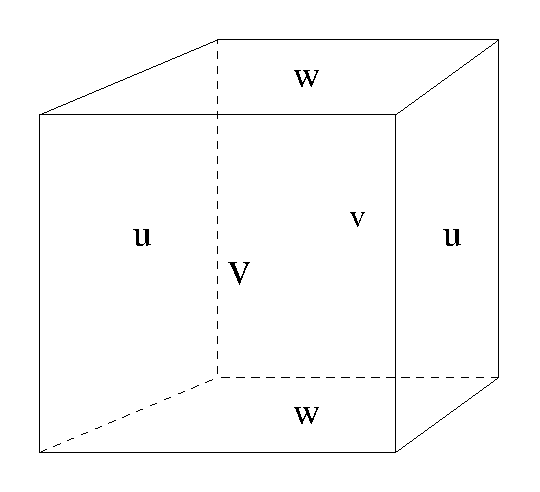
\includegraphics{part2/cgrid3d.eps}} }
\label{fig-cgrid3d}
\caption{Three dimensional staggering of velocity components. This
facilitates the natural discretization of the continuity and tracer
equations. }
\end{figure}

\subsection{Horizontal grid}

\begin{figure}
\centerline{ \begin{tabular}{cc}
  \resizebox{!}{2in}{ 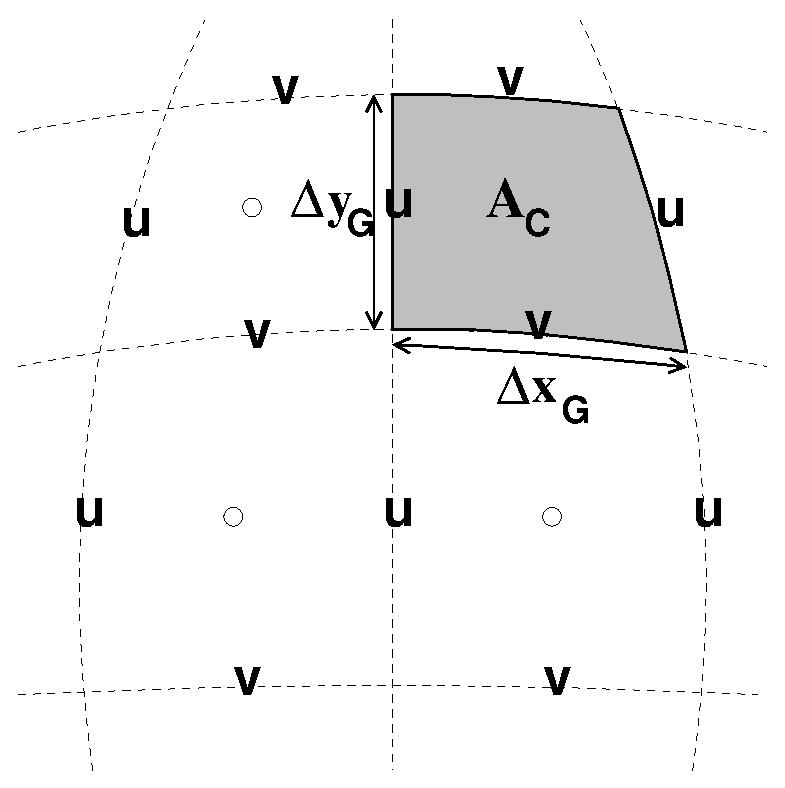
\includegraphics{part2/hgrid-Ac.eps}}
& \resizebox{!}{2in}{ 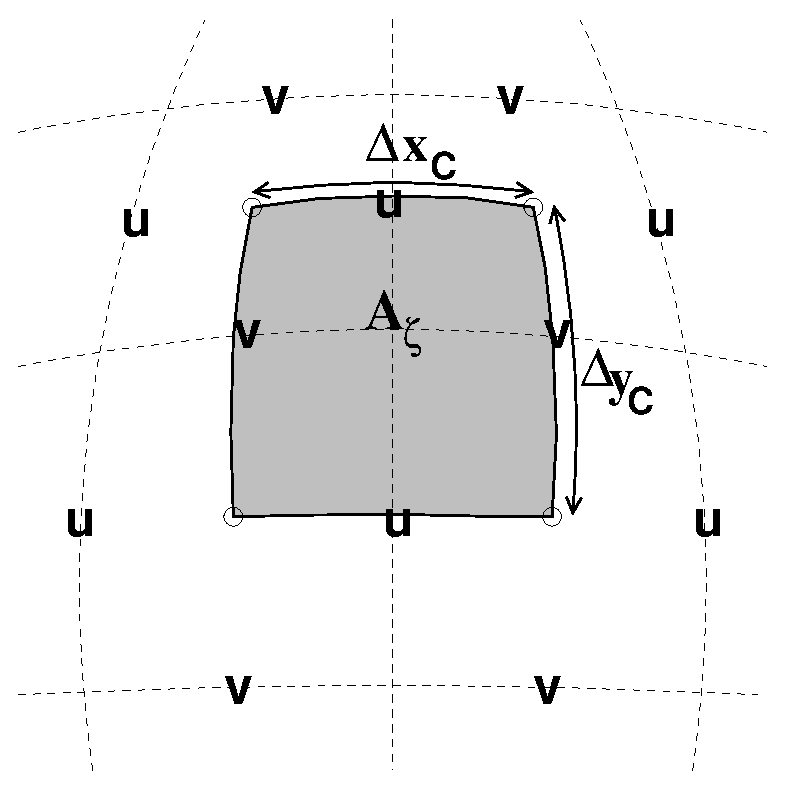
\includegraphics{part2/hgrid-Az.eps}}
\\
  \resizebox{!}{2in}{ 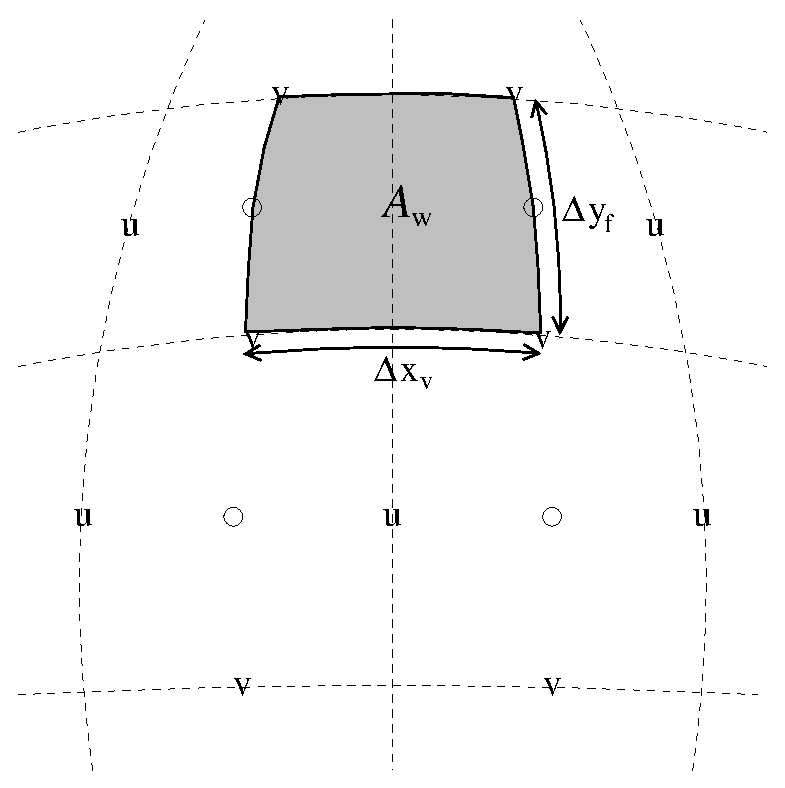
\includegraphics{part2/hgrid-Au.eps}}
& \resizebox{!}{2in}{ 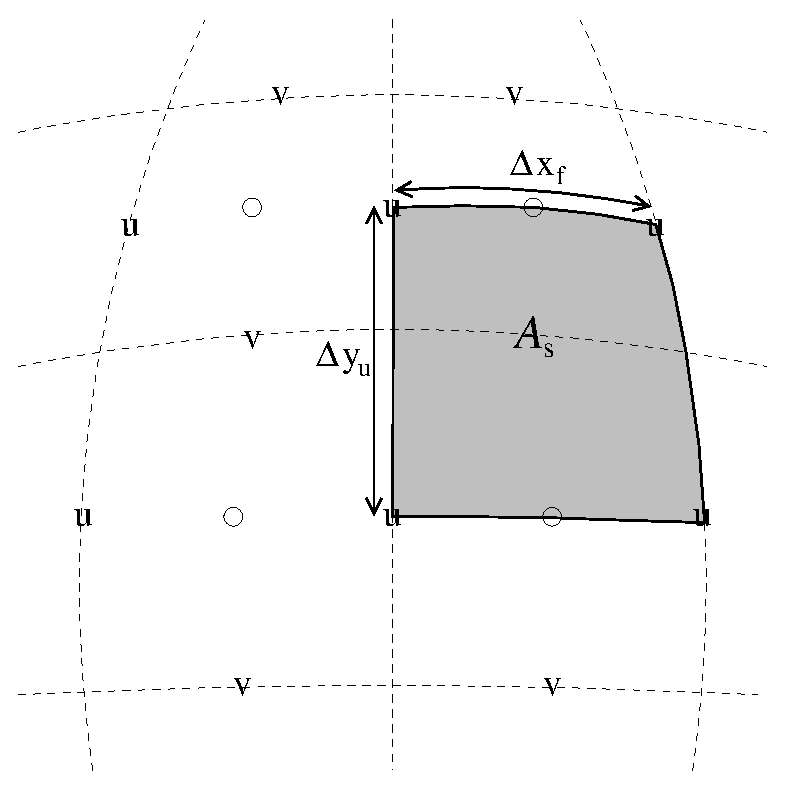
\includegraphics{part2/hgrid-Av.eps}}
\end{tabular} }
\label{fig-hgrid}
\caption{Three dimensional staggering of velocity components. This
facilitates the natural discretization of the continuity and tracer
equations. }
\end{figure}

\subsection{Vertical grid}

\begin{figure}
\centerline{ \begin{tabular}{cc}
  \raisebox{4in}{a)}
  \resizebox{!}{4in}{ 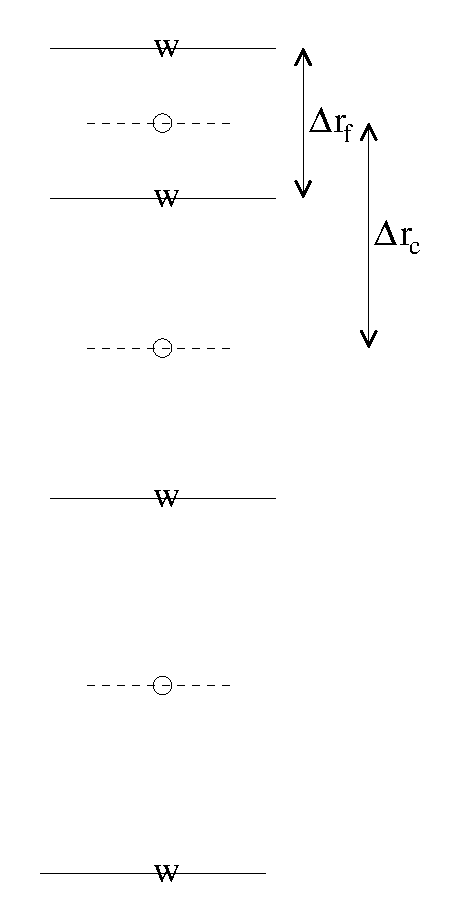
\includegraphics{part2/vgrid-cellcentered.eps}}
&
 \raisebox{4in}{b)}
 \resizebox{!}{4in}{ 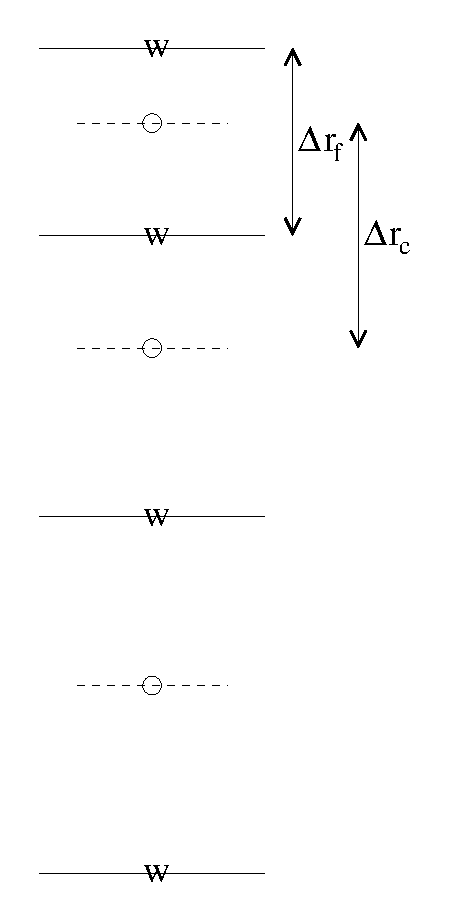
\includegraphics{part2/vgrid-accurate.eps}}
\end{tabular} }
\label{fig-vgrid}
\caption{Two versions of the vertical grid. a) The cell centered
approach where the interface depths are specified and the tracer
points centered in between the interfaces. b) The interface centered
approach where tracer levels are specified and the w-interfaces are
centered in between.}
\end{figure}


\subsection{Continuity and horizontal pressure gradient terms}

The core algorithm is based on the ``C grid'' discretization of the
continuity equation which can be summarized as:
\begin{eqnarray}
\partial_t u + \frac{1}{\Delta x_c} \delta_i \left. \frac{ \partial \Phi}{\partial r}\right|_{s} \eta + \frac{\epsilon_{nh}}{\Delta x_c} \delta_i \Phi_{nh}' & = & G_u - \frac{1}{\Delta x_c} \delta_i \Phi_h' \\
\partial_t v + \frac{1}{\Delta y_c} \delta_j \left. \frac{ \partial \Phi}{\partial r}\right|_{s} \eta + \frac{\epsilon_{nh}}{\Delta y_c} \delta_j \Phi_{nh}' & = & G_v - \frac{1}{\Delta y_c} \delta_j \Phi_h' \\
\epsilon_{nh} \left( \partial_t w + \frac{1}{\Delta r_c} \delta_k \Phi_{nh}' \right) & = & \epsilon_{nh} G_w + \overline{b}^k - \frac{1}{\Delta r_c} \delta_k \Phi_{h}' \\
\delta_i \Delta y_g \Delta r_f h_w u +
\delta_j \Delta x_g \Delta r_f h_s v +
\delta_k {\cal A}_c w & = & {\cal A}_c \delta_k (P-E)_{r=0}
\end{eqnarray}
where the continuity equation has been most naturally discretized by
staggering the three components of velocity as shown in
Fig.~\ref{fig-cgrid3d}. The grid lengths $\Delta x_c$ and $\Delta y_c$
are the lengths between tracer points (cell centers). The grid lengths
$\Delta x_g$, $\Delta y_g$ are the grid lengths between cell
corners. $\Delta r_f$ and $\Delta r_c$ are the distance (in units of
$r$) between level interfaces (w-level) and level centers (tracer
level). The surface area presented in the vertical is denoted ${\cal
A}_c$.  The factors $h_w$ and $h_s$ are non-dimensional fractions
(between 0 and 1) that represent the fraction cell depth that is
``open'' for fluid flow.
\marginpar{$h_w$: {\bf hFacW}}
\marginpar{$h_s$: {\bf hFacS}}

The last equation, the discrete continuity equation, can be summed in
the vertical to yeild the free-surface equation:
\begin{equation}
{\cal A}_c \partial_t \eta + \delta_i \sum_k \Delta y_g \Delta r_f h_w u + \delta_j \sum_k \Delta x_g \Delta r_f h_s v =
{\cal A}_c(P-E)_{r=0}
\end{equation}
The source term $P-E$ on the rhs of continuity accounts for the local
addition of volume due to excess precipitation and run-off over
evaporation and only enters the top-level of the {\em ocean} model.

\subsection{Hydrostatic balance}

The vertical momentum equation has the hydrostatic or
quasi-hydrostatic balance on the right hand side. This discretization
guarantees that the conversion of potential to kinetic energy as
derived from the buoyancy equation exactly matches the form derived
from the pressure gradient terms when forming the kinetic energy
equation.

In the ocean, using z-ccordinates, the hydrostatic balance terms are
discretized:
\begin{equation}
\epsilon_{nh} \partial_t w
+ g \overline{\rho'}^k + \frac{1}{\Delta z} \delta_k \Phi_h' = \ldots
\end{equation}

In the atmosphere, using p-coordinates, hydrostatic balance is
discretized:
\begin{equation}
\overline{\theta'}^k + \frac{1}{\Delta \Pi} \delta_k \Phi_h' = 0
\end{equation}
where $\Delta \Pi$ is the difference in Exner function between the
pressure points. The non-hydrostatic equations are not available in
the atmosphere.

The difference in approach between ocean and atmosphere occurs because
of the direct use of the ideal gas equation in forming the potential
energy conversion term $\alpha \omega$. The form of these consversion
terms is discussed at length in \cite{Adcroft01}.

Because of the different representation of hydrostatic balance between
ocean and atmosphere there is no elegant way to represent both systems
using an arbitrary coordinate.

The integration for hydrostatic pressure is made in the positive $r$
direction (increasing k-index). For the ocean, this is from the
free-surface down and for the atmosphere this is from the ground up.

The calculations are made in the subroutine {\em
CALC\_PHI\_HYD}. Inside this routine, one of other of the
atmospheric/oceanic form is selected based on the string variable {\bf
buoyancyRelation}.

\subsection{Flux-form momentum equations}

The original finite volume model was based on the Eulerian flux form
momentum equations. This is the default though the vector invariant
form is optionally available (and recommended in some cases).

The ``G's'' (our colloquial name for all terms on rhs!) are broken
into the various advective, Coriolis, horizontal dissipation, vertical
dissipation and metric forces:
\marginpar{$G_u$: {\bf Gu} }
\marginpar{$G_v$: {\bf Gv} }
\marginpar{$G_w$: {\bf Gw} }
\begin{eqnarray}
G_u & = & G_u^{adv} + G_u^{cor} + G_u^{h-diss} + G_u^{v-diss} +
G_u^{metric} + G_u^{nh-metric} \\
G_v & = & G_v^{adv} + G_v^{cor} + G_v^{h-diss} + G_v^{v-diss} +
G_v^{metric} + G_v^{nh-metric} \\
G_w & = & G_w^{adv} + G_w^{cor} + G_w^{h-diss} + G_w^{v-diss} +
G_w^{metric} + G_w^{nh-metric}
\end{eqnarray}
In the hydrostatic limit, $G_w=0$ and $\epsilon_{nh}=0$, reducing the
vertical momentum to hydrostatic balance.

These terms are calculated in routines called from subroutine {\em
CALC\_MOM\_RHS} a collected into the global arrays {\bf Gu}, {\bf Gv},
and {\bf Gw}.

\fbox{ \begin{minipage}{4.25in}
{\em S/R CALC\_MOM\_RHS} ({\em pkg/mom\_fluxform/calc\_mom\_rhs.F})

$G_u$: {\bf Gu} ({\em DYNVARS.h})

$G_v$: {\bf Gv} ({\em DYNVARS.h})

$G_w$: {\bf Gw} ({\em DYNVARS.h})
\end{minipage} }


\subsubsection{Advection of momentum}

The advective operator is second order accurate in space:
\begin{eqnarray}
{\cal A}_w \Delta r_f h_w G_u^{adv} & = &
  \delta_i \overline{ U }^i \overline{ u }^i
+ \delta_j \overline{ V }^i \overline{ u }^j
+ \delta_k \overline{ W }^i \overline{ u }^k \\
{\cal A}_s \Delta r_f h_s G_v^{adv} & = &
  \delta_i \overline{ U }^j \overline{ v }^i
+ \delta_j \overline{ V }^j \overline{ v }^j
+ \delta_k \overline{ W }^j \overline{ v }^k \\
{\cal A}_c \Delta r_c G_w^{adv} & = &
  \delta_i \overline{ U }^k \overline{ w }^i
+ \delta_j \overline{ V }^k \overline{ w }^j
+ \delta_k \overline{ W }^k \overline{ w }^k \\
\end{eqnarray}
and because of the flux form does not contribute to the global budget
of linear momentum. The quantities $U$, $V$ and $W$ are volume fluxes
defined:
\marginpar{$U$: {\bf uTrans} }
\marginpar{$V$: {\bf vTrans} }
\marginpar{$W$: {\bf rTrans} }
\begin{eqnarray}
U & = & \Delta y_g \Delta r_f h_w u \\
V & = & \Delta x_g \Delta r_f h_s v \\
W & = & {\cal A}_c w
\end{eqnarray}
The advection of momentum takes the same form as the advection of
tracers but by a translated advective flow. Consequently, the
conservation of second moments, derived for tracers later, applies to
$u^2$ and $v^2$ and $w^2$ so that advection of momentum correctly
conserves kinetic energy.

\fbox{ \begin{minipage}{4.25in}
{\em S/R MOM\_U\_ADV\_UU} ({\em mom\_u\_adv\_uu.F})

{\em S/R MOM\_U\_ADV\_VU} ({\em mom\_u\_adv\_vu.F})

{\em S/R MOM\_U\_ADV\_WU} ({\em mom\_u\_adv\_wu.F})

{\em S/R MOM\_U\_ADV\_UV} ({\em mom\_u\_adv\_uv.F})

{\em S/R MOM\_U\_ADV\_VV} ({\em mom\_u\_adv\_vv.F})

{\em S/R MOM\_U\_ADV\_WV} ({\em mom\_u\_adv\_wv.F})

$uu$, $uv$, $vu$, $vv$: {\bf aF} (local to {\em calc\_mom\_rhs.F})
\end{minipage} }



\subsubsection{Coriolis terms}

The ``pure C grid'' Coriolis terms (i.e. in absence of C-D scheme) are
discretized:
\begin{eqnarray}
{\cal A}_w \Delta r_f h_w G_u^{Cor} & = &
  \overline{ f {\cal A}_c \Delta r_f h_c \overline{ v }^j }^i
- \epsilon_{nh} \overline{ f' {\cal A}_c \Delta r_f h_c \overline{ w }^k }^i \\
{\cal A}_s \Delta r_f h_s G_v^{Cor} & = &
- \overline{ f {\cal A}_c \Delta r_f h_c \overline{ u }^i }^j \\
{\cal A}_c \Delta r_c G_w^{Cor} & = &
 \epsilon_{nh} \overline{ f' {\cal A}_c \Delta r_f h_c \overline{ u }^i }^k
\end{eqnarray}
where the Coriolis parameters $f$ and $f'$ are defined:
\begin{eqnarray}
f & = & 2 \Omega \sin{\phi} \\
f' & = & 2 \Omega \cos{\phi}
\end{eqnarray}
when using spherical geometry, otherwise the $\beta$-plane definition is used:
\begin{eqnarray}
f & = & f_o + \beta y \\
f' & = & 0
\end{eqnarray}

This discretization globally conserves kinetic energy. It should be
noted that despite the use of this discretization in former
publications, all calculations to date have used the following
different discretization:
\begin{eqnarray}
G_u^{Cor} & = &
  f_u \overline{ v }^{ji}
- \epsilon_{nh} f_u' \overline{ w }^{ik} \\
G_v^{Cor} & = &
- f_v \overline{ u }^{ij} \\
G_w^{Cor} & = &
 \epsilon_{nh} f_w' \overline{ u }^{ik}
\end{eqnarray}
\marginpar{Need to change the default in code to match this}
where the subscripts on $f$ and $f'$ indicate evaluation of the
Coriolis parameters at the appropriate points in space. The above
discretization does {\em not} conserve anything, especially energy. An
option to recover this discretization has been retained for backward
compatibility testing (set run-time logical {\bf
useNonconservingCoriolis} to {\em true} which otherwise defaults to
{\em false}).

\fbox{ \begin{minipage}{4.25in}
{\em S/R MOM\_CDSCHEME} ({\em mom\_cdscheme.F})

{\em S/R MOM\_U\_CORIOLIS} ({\em mom\_u\_coriolis.F})

{\em S/R MOM\_V\_CORIOLIS} ({\em mom\_v\_coriolis.F})

$G_u^{Cor}$, $G_v^{Cor}$: {\bf cF} (local to {\em calc\_mom\_rhs.F})
\end{minipage} }


\subsubsection{Curvature metric terms}

The most commonly used coordinate system on the sphere is the
geographic system $(\lambda,\phi)$. The curvilinear nature of these
coordinates on the sphere lead to some ``metric'' terms in the
component momentum equations. Under the thin-atmosphere and
hydrostatic approximations these terms are discretized:
\begin{eqnarray}
{\cal A}_w \Delta r_f h_w G_u^{metric} & = &
  \overline{ \frac{ \overline{u}^i }{a} \tan{\phi} {\cal A}_c \Delta r_f h_c \overline{ v }^j }^i \\
{\cal A}_s \Delta r_f h_s G_v^{metric} & = &
- \overline{ \frac{ \overline{u}^i }{a} \tan{\phi} {\cal A}_c \Delta r_f h_c \overline{ u }^i }^j \\
G_w^{metric} & = & 0
\end{eqnarray}
where $a$ is the radius of the planet (sphericity is assumed) or the
radial distance of the particle (i.e. a function of height).  It is
easy to see that this discretization satisfies all the properties of
the discrete Coriolis terms since the metric factor $\frac{u}{a}
\tan{\phi}$ can be viewed as a modification of the vertical Coriolis
parameter: $f \rightarrow f+\frac{u}{a} \tan{\phi}$.

However, as for the Coriolis terms, a non-energy conserving form has
exclusively been used to date:
\begin{eqnarray}
G_u^{metric} & = & \frac{u \overline{v}^{ij} }{a} \tan{\phi} \\
G_v^{metric} & = & \frac{ \overline{u}^{ij} \overline{u}^{ij}}{a} \tan{\phi}
\end{eqnarray}
where $\tan{\phi}$ is evaluated at the $u$ and $v$ points
respectively.

\fbox{ \begin{minipage}{4.25in}
{\em S/R MOM\_U\_METRIC\_SPHERE} ({\em mom\_u\_metric\_sphere.F})

{\em S/R MOM\_V\_METRIC\_SPHERE} ({\em mom\_v\_metric\_sphere.F})

$G_u^{metric}$, $G_v^{metric}$: {\bf mT} (local to {\em calc\_mom\_rhs.F})
\end{minipage} }



\subsubsection{Non-hydrostatic metric terms}

For the non-hydrostatic equations, dropping the thin-atmosphere
approximation re-introduces metric terms involving $w$ and are
required to conserve anglular momentum:
\begin{eqnarray}
{\cal A}_w \Delta r_f h_w G_u^{metric} & = &
- \overline{ \frac{ \overline{u}^i \overline{w}^k }{a} {\cal A}_c \Delta r_f h_c }^i \\
{\cal A}_s \Delta r_f h_s G_v^{metric} & = &
- \overline{ \frac{ \overline{v}^j \overline{w}^k }{a} {\cal A}_c \Delta r_f h_c}^j \\
{\cal A}_c \Delta r_c G_w^{metric} & = &
  \overline{ \frac{ {\overline{u}^i}^2 + {\overline{v}^j}^2}{a} {\cal A}_c \Delta r_f h_c }^k
\end{eqnarray}

Because we are always consistent, even if consistently wrong, we have,
in the past, used a different discretization in the model which is:
\begin{eqnarray}
G_u^{metric} & = &
- \frac{u}{a} \overline{w}^{ik} \\
G_v^{metric} & = &
- \frac{v}{a} \overline{w}^{jk} \\
G_w^{metric} & = &
  \frac{1}{a} ( {\overline{u}^{ik}}^2 + {\overline{v}^{jk}}^2 )
\end{eqnarray}

\fbox{ \begin{minipage}{4.25in}
{\em S/R MOM\_U\_METRIC\_NH} ({\em mom\_u\_metric\_nh.F})

{\em S/R MOM\_V\_METRIC\_NH} ({\em mom\_v\_metric\_nh.F})

$G_u^{metric}$, $G_v^{metric}$: {\bf mT} (local to {\em calc\_mom\_rhs.F})
\end{minipage} }


\subsubsection{Lateral dissipation}

Historically, we have represented the SGS Reynolds stresses as simply
down gradient momentum fluxes, ignoring constraints on the stress
tensor such as symmetry.
\begin{eqnarray}
{\cal A}_w \Delta r_f h_w G_u^{h-diss} & = &
  \delta_i  \Delta y_f \Delta r_f h_c \tau_{11}
+ \delta_j  \Delta x_v \Delta r_f h_\zeta \tau_{12} \\
{\cal A}_s \Delta r_f h_s G_v^{h-diss} & = &
  \delta_i  \Delta y_u \Delta r_f h_\zeta \tau_{21}
+ \delta_j  \Delta x_f \Delta r_f h_c \tau_{22}
\end{eqnarray}
\marginpar{Check signs of stress definitions}

The lateral viscous stresses are discretized:
\begin{eqnarray}
\tau_{11} & = & A_h c_{11\Delta}(\phi) \frac{1}{\Delta x_f} \delta_i u
               -A_4 c_{11\Delta^2}(\phi) \frac{1}{\Delta x_f} \delta_i \nabla^2 u \\
\tau_{12} & = & A_h c_{12\Delta}(\phi) \frac{1}{\Delta y_u} \delta_j u
               -A_4 c_{12\Delta^2}(\phi)\frac{1}{\Delta y_u} \delta_j \nabla^2 u \\
\tau_{21} & = & A_h c_{21\Delta}(\phi) \frac{1}{\Delta x_v} \delta_i v
               -A_4 c_{21\Delta^2}(\phi) \frac{1}{\Delta x_v} \delta_i \nabla^2 v \\
\tau_{22} & = & A_h c_{22\Delta}(\phi) \frac{1}{\Delta y_f} \delta_j v
               -A_4 c_{22\Delta^2}(\phi) \frac{1}{\Delta y_f} \delta_j \nabla^2 v
\end{eqnarray}
where the non-dimensional factors $c_{lm\Delta^n}(\phi), \{l,m,n\} \in
\{1,2\}$ define the ``cosine'' scaling with latitude which can be
applied in various ad-hoc ways. For instance, $c_{11\Delta} =
c_{21\Delta} = (\cos{\phi})^{3/2}$, $c_{12\Delta}=c_{22\Delta}=0$ would
represent the an-isotropic cosine scaling typically used on the
``lat-lon'' grid for Laplacian viscosity.
\marginpar{Need to tidy up method for controlling this in code}

It should be noted that dispite the ad-hoc nature of the scaling, some
scaling must be done since on a lat-lon grid the converging meridians
make it very unlikely that a stable viscosity parameter exists across
the entire model domain.

The Laplacian viscosity coefficient, $A_h$ ({\bf viscAh}), has units
of $m^2 s^{-1}$. The bi-harmonic viscosity coefficient, $A_4$ ({\bf
viscA4}), has units of $m^4 s^{-1}$.

\fbox{ \begin{minipage}{4.25in}
{\em S/R MOM\_U\_XVISCFLUX} ({\em mom\_u\_xviscflux.F})

{\em S/R MOM\_U\_YVISCFLUX} ({\em mom\_u\_yviscflux.F})

{\em S/R MOM\_V\_XVISCFLUX} ({\em mom\_v\_xviscflux.F})

{\em S/R MOM\_V\_YVISCFLUX} ({\em mom\_v\_yviscflux.F})

$\tau_{11}$, $\tau_{12}$, $\tau_{22}$, $\tau_{22}$: {\bf vF}, {\bf
v4F} (local to {\em calc\_mom\_rhs.F})
\end{minipage} }

Two types of lateral boundary condition exist for the lateral viscous
terms, no-slip and free-slip.

The free-slip condition is most convenient to code since it is
equivalent to zero-stress on boundaries. Simple masking of the stress
components sets them to zero. The fractional open stress is properly
handled using the lopped cells.

The no-slip condition defines the normal gradient of a tangential flow
such that the flow is zero on the boundary. Rather than modify the
stresses by using complicated functions of the masks and ``ghost''
points (see \cite{Adcroft+Marshall98}) we add the boundary stresses as
an additional source term in cells next to solid boundaries. This has
the advantage of being able to cope with ``thin walls'' and also makes
the interior stress calculation (code) independent of the boundary
conditions. The ``body'' force takes the form:
\begin{eqnarray}
G_u^{side-drag} & = &
\frac{4}{\Delta z_f} \overline{ (1-h_\zeta) \frac{\Delta x_v}{\Delta y_u} }^j
\left( A_h c_{12\Delta}(\phi) u - A_4 c_{12\Delta^2}(\phi) \nabla^2 u \right)
\\
G_v^{side-drag} & = &
\frac{4}{\Delta z_f} \overline{ (1-h_\zeta) \frac{\Delta y_u}{\Delta x_v} }^i
\left( A_h c_{21\Delta}(\phi) v - A_4 c_{21\Delta^2}(\phi) \nabla^2 v \right)
\end{eqnarray}

In fact, the above discretization is not quite complete because it
assumes that the bathymetry at velocity points is deeper than at
neighbouring vorticity points, e.g. $1-h_w < 1-h_\zeta$

\fbox{ \begin{minipage}{4.25in}
{\em S/R MOM\_U\_SIDEDRAG} ({\em mom\_u\_sidedrag.F})

{\em S/R MOM\_V\_SIDEDRAG} ({\em mom\_v\_sidedrag.F})

$G_u^{side-drag}$, $G_v^{side-drag}$: {\bf vF} (local to {\em calc\_mom\_rhs.F})
\end{minipage} }


\subsubsection{Vertical dissipation}

Vertical viscosity terms are discretized with only partial adherence
to the variable grid lengths introduced by the finite volume
formulation. This reduces the formal accuracy of these terms to just
first order but only next to boundaries; exactly where other terms
appear such as linar and quadratic bottom drag.
\begin{eqnarray}
G_u^{v-diss} & = &
\frac{1}{\Delta r_f h_w} \delta_k \tau_{13} \\
G_v^{v-diss} & = &
\frac{1}{\Delta r_f h_s} \delta_k \tau_{23} \\
G_w^{v-diss} & = & \epsilon_{nh}
\frac{1}{\Delta r_f h_d} \delta_k \tau_{33}
\end{eqnarray}
represents the general discrete form of the vertical dissipation terms.

In the interior the vertical stresses are discretized:
\begin{eqnarray}
\tau_{13} & = & A_v \frac{1}{\Delta r_c} \delta_k u \\
\tau_{23} & = & A_v \frac{1}{\Delta r_c} \delta_k v \\
\tau_{33} & = & A_v \frac{1}{\Delta r_f} \delta_k w
\end{eqnarray}
It should be noted that in the non-hydrostatic form, the stress tensor
is even less consistent than for the hydrostatic (see Wazjowicz
\cite{Waojz}). It is well known how to do this properly (see Griffies
\cite{Griffies}) and is on the list of to-do's.

\fbox{ \begin{minipage}{4.25in}
{\em S/R MOM\_U\_RVISCLFUX} ({\em mom\_u\_rviscflux.F})

{\em S/R MOM\_V\_RVISCLFUX} ({\em mom\_v\_rviscflux.F})

$\tau_{13}$: {\bf urf} (local to {\em calc\_mom\_rhs.F})

$\tau_{23}$: {\bf vrf} (local to {\em calc\_mom\_rhs.F})
\end{minipage} }


As for the lateral viscous terms, the free-slip condition is
equivalent to simply setting the stress to zero on boundaries.  The
no-slip condition is implemented as an additional term acting on top
of the interior and free-slip stresses. Bottom drag represents
additional friction, in addition to that imposed by the no-slip
condition at the bottom. The drag is cast as a stress expressed as a
linear or quadratic function of the mean flow in the layer above the
topography:
\begin{eqnarray}
\tau_{13}^{bottom-drag} & = &
\left(
2 A_v \frac{1}{\Delta r_c}
+ r_b
+ C_d \sqrt{ \overline{2 KE}^i }
\right) u \\
\tau_{23}^{bottom-drag} & = &
\left(
2 A_v \frac{1}{\Delta r_c}
+ r_b
+ C_d \sqrt{ \overline{2 KE}^j }
\right) v
\end{eqnarray}
where these terms are only evaluated immediately above topography.
$r_b$ ({\bf bottomDragLinear}) has units of $m s^{-1}$ and a typical value
of the order 0.0002 $m s^{-1}$. $C_d$ ({\bf bottomDragQuadratic}) is
dimensionless with typical values in the range 0.001--0.003.

\fbox{ \begin{minipage}{4.25in}
{\em S/R MOM\_U\_BOTTOMDRAG} ({\em mom\_u\_bottomdrag.F})

{\em S/R MOM\_V\_BOTTOMDRAG} ({\em mom\_v\_bottomdrag.F})

$\tau_{13}^{bottom-drag}$, $\tau_{23}^{bottom-drag}$: {\bf vf} (local to {\em calc\_mom\_rhs.F})
\end{minipage} }





\subsection{Tracer equations}

The tracer equations are discretized consistantly with the continuity
equation to facilitate conservation properties analogous to the
continuum:
\begin{equation}
{\cal A}_c \Delta r_f h_c \partial_\theta
+ \delta_i U \overline{ \theta }^i
+ \delta_j V \overline{ \theta }^j
+ \delta_k W \overline{ \theta }^k
= {\cal A}_c \Delta r_f h_c {\cal S}_\theta + \theta {\cal A}_c \delta_k (P-E)_{r=0}
\end{equation}
The quantities $U$, $V$ and $W$ are volume fluxes defined:
\marginpar{$U$: {\bf uTrans} }
\marginpar{$V$: {\bf vTrans} }
\marginpar{$W$: {\bf rTrans} }
\begin{eqnarray}
U & = & \Delta y_g \Delta r_f h_w u \\
V & = & \Delta x_g \Delta r_f h_s v \\
W & = & {\cal A}_c w
\end{eqnarray}
${\cal S}$ represents the ``parameterized'' SGS processes and
physics associated with the tracer. For instance, potential
temperature equation in the ocean has is forced by surface and
partially penetrating heat fluxes:
\begin{equation}
{\cal A}_c \Delta r_f h_c {\cal S}_\theta = \frac{1}{c_p \rho_o} \delta_k {\cal A}_c {\cal Q}
\end{equation}
while the salt equation has no real sources, ${\cal S}=0$, which
leaves just the $P-E$ term.

The continuity equation can be recovered by setting ${\cal Q}=0$ and
$\theta=1$. The term $\theta (P-E)_{r=0}$ is required to retain local
conservation of $\theta$. Global conservation is not possible using
the flux-form (as here) and a linearized free-surface
(\cite{Griffies00,Campin02}).




\subsection{Derivation of discrete energy conservation}

These discrete equations conserve kinetic plus potential energy using the
following definitions:
\begin{equation}
KE = \frac{1}{2} \left( \overline{ u^2 }^i + \overline{ v^2 }^j +
\epsilon_{nh} \overline{ w^2 }^k \right)
\end{equation}


\subsection{Vector invariant momentum equations}

The finite volume method lends itself to describing the continuity and
tracer equations in curvilinear coordinate systems but the appearance
of new metric terms in the flux-form momentum equations makes
generalizing them far from elegant. The vector invariant form of the
momentum equations are exactly that; invariant under coordinate
transformations.

The non-hydrostatic vector invariant equations read:
\begin{equation}
\partial_t \vec{v} + ( 2\vec{\Omega} + \vec{\zeta}) \wedge \vec{v}
- b \hat{r}
+ \vec{\nabla} B = \vec{\nabla} \cdot \vec{\bf \tau}
\end{equation}
which describe motions in any orthogonal curvilinear coordinate
system. Here, $B$ is the Bernoulli function and $\vec{\zeta}=\nabla
\wedge \vec{v}$ is the vorticity vector. We can take advantage of the
elegance of these equations when discretizing them and use the
discrete definitions of the grad, curl and divergence operators to
satisfy constraints. We can also consider the analogy to forming
derived equations, such as the vorticity equation, and examine how the
discretization can be adjusted to give suitable vorticity advection
among other things.

The underlying algorithm is the same as for the flux form
equations. All that has changed is the contents of the ``G's''. For
the time-being, only the hydrostatic terms have been coded but we will
indicate the points where non-hydrostatic contributions will enter:
\begin{eqnarray}
G_u & = & G_u^{fv} + G_u^{\zeta_3 v} + G_u^{\zeta_2 w} + G_u^{\partial_x B}
+ G_u^{\partial_z \tau^x} + G_u^{h-dissip} + G_u^{v-dissip} \\
G_v & = & G_v^{fu} + G_v^{\zeta_3 u} + G_v^{\zeta_1 w} + G_v^{\partial_y B}
+ G_v^{\partial_z \tau^y} + G_v^{h-dissip} + G_v^{v-dissip} \\
G_w & = & G_w^{fu} + G_w^{\zeta_1 v} + G_w^{\zeta_2 u} + G_w^{\partial_z B}
+ G_w^{h-dissip} + G_w^{v-dissip}
\end{eqnarray}

\fbox{ \begin{minipage}{4.25in}
{\em S/R CALC\_MOM\_RHS} ({\em pkg/mom\_vecinv/calc\_mom\_rhs.F})

$G_u$: {\bf Gu} ({\em DYNVARS.h})

$G_v$: {\bf Gv} ({\em DYNVARS.h})

$G_w$: {\bf Gw} ({\em DYNVARS.h})
\end{minipage} }

\subsubsection{Relative vorticity}

The vertical component of relative vorticity is explicitly calculated
and use in the discretization. The particular form is crucial for
numerical stablility; alternative definitions break the conservation
properties of the discrete equations.

Relative vorticity is defined:
\begin{equation}
\zeta_3 = \frac{\Gamma}{A_\zeta}
= \frac{1}{{\cal A}_\zeta} ( \delta_i \Delta y_c v - \delta_j \Delta x_c u )
\end{equation}
where ${\cal A}_\zeta$ is the area of the vorticity cell presented in
the vertical and $\Gamma$ is the circulation about that cell.

\fbox{ \begin{minipage}{4.25in}
{\em S/R MOM\_VI\_CALC\_RELVORT3} ({\em mom\_vi\_calc\_relvort3.F})

$\zeta_3$: {\bf vort3} (local to {\em calc\_mom\_rhs.F})
\end{minipage} }


\subsubsection{Kinetic energy}

The kinetic energy, denoted $KE$, is defined:
\begin{equation}
KE = \frac{1}{2} ( \overline{ u^2 }^i + \overline{ v^2 }^j 
+ \epsilon_{nh} \overline{ w^2 }^k )
\end{equation}

\fbox{ \begin{minipage}{4.25in}
{\em S/R MOM\_VI\_CALC\_KE} ({\em mom\_vi\_calc\_ke.F})

$KE$: {\bf KE} (local to {\em calc\_mom\_rhs.F})
\end{minipage} }


\subsubsection{Coriolis terms}

The potential enstrophy conserving form of the linear Coriolis terms
are written:
\begin{eqnarray}
G_u^{fv} & = &
\frac{1}{\Delta x_c}
\overline{ \frac{f}{h_\zeta} }^j \overline{ \overline{ \Delta x_g h_s v }^j }^i \\
G_v^{fu} & = & -
\frac{1}{\Delta y_c}
\overline{ \frac{f}{h_\zeta} }^i \overline{ \overline{ \Delta y_g h_w u }^i }^j
\end{eqnarray}
Here, the Coriolis parameter $f$ is defined at vorticity (corner)
points.
\marginpar{$f$: {\bf fCoriG}}
\marginpar{$h_\zeta$: {\bf hFacZ}}

The potential enstrophy conserving form of the non-linear Coriolis
terms are written:
\begin{eqnarray}
G_u^{\zeta_3 v} & = &
\frac{1}{\Delta x_c}
\overline{ \frac{\zeta_3}{h_\zeta} }^j \overline{ \overline{ \Delta x_g h_s v }^j }^i \\
G_v^{\zeta_3 u} & = & -
\frac{1}{\Delta y_c}
\overline{ \frac{\zeta_3}{h_\zeta} }^i \overline{ \overline{ \Delta y_g h_w u }^i }^j
\end{eqnarray}
\marginpar{$\zeta_3$: {\bf vort3}}

The Coriolis terms can also be evaluated together and expressed in
terms of absolute vorticity $f+\zeta_3$. The potential enstrophy
conserving form using the absolute vorticity is written:
\begin{eqnarray}
G_u^{fv} + G_u^{\zeta_3 v} & = &
\frac{1}{\Delta x_c}
\overline{ \frac{f + \zeta_3}{h_\zeta} }^j \overline{ \overline{ \Delta x_g h_s v }^j }^i \\
G_v^{fu} + G_v^{\zeta_3 u} & = & -
\frac{1}{\Delta y_c}
\overline{ \frac{f + \zeta_3}{h_\zeta} }^i \overline{ \overline{ \Delta y_g h_w u }^i }^j
\end{eqnarray}

\marginpar{Run-time control needs to be added for these options} The
disctinction between using absolute vorticity or relative vorticity is
useful when constructing higher order advection schemes; monotone
advection of relative vorticity behaves differently to monotone
advection of absolute vorticity. Currently the choice of
relative/absolute vorticity, centered/upwind/high order advection is
available only through commented subroutine calls.

\fbox{ \begin{minipage}{4.25in}
{\em S/R MOM\_VI\_CORIOLIS} ({\em mom\_vi\_coriolis.F})

{\em S/R MOM\_VI\_U\_CORIOLIS} ({\em mom\_vi\_u\_coriolis.F})

{\em S/R MOM\_VI\_V\_CORIOLIS} ({\em mom\_vi\_v\_coriolis.F})

$G_u^{fv}$, $G_u^{\zeta_3 v}$: {\bf uCf} (local to {\em calc\_mom\_rhs.F})

$G_v^{fu}$, $G_v^{\zeta_3 u}$: {\bf vCf} (local to {\em calc\_mom\_rhs.F})
\end{minipage} }


\subsubsection{Shear terms}

The shear terms ($\zeta_2w$ and $\zeta_1w$) are are discretized to
guarantee that no spurious generation of kinetic energy is possible;
the horizontal gradient of Bernoulli function has to be consistent
with the vertical advection of shear:
\marginpar{N-H terms have not been tried!}
\begin{eqnarray}
G_u^{\zeta_2 w} & = &
\frac{1}{ {\cal A}_w \Delta r_f h_w } \overline{
\overline{ {\cal A}_c w }^i ( \delta_k u - \epsilon_{nh} \delta_j w )
}^k \\
G_v^{\zeta_1 w} & = &
\frac{1}{ {\cal A}_s \Delta r_f h_s } \overline{
\overline{ {\cal A}_c w }^i ( \delta_k u - \epsilon_{nh} \delta_j w )
}^k
\end{eqnarray}

\fbox{ \begin{minipage}{4.25in}
{\em S/R MOM\_VI\_U\_VERTSHEAR} ({\em mom\_vi\_u\_vertshear.F})

{\em S/R MOM\_VI\_V\_VERTSHEAR} ({\em mom\_vi\_v\_vertshear.F})

$G_u^{\zeta_2 w}$: {\bf uCf} (local to {\em calc\_mom\_rhs.F})

$G_v^{\zeta_1 w}$: {\bf vCf} (local to {\em calc\_mom\_rhs.F})
\end{minipage} }



\subsubsection{Gradient of Bernoulli function}

\begin{eqnarray}
G_u^{\partial_x B} & = &
\frac{1}{\Delta x_c} \delta_i ( \phi' + KE ) \\
G_v^{\partial_y B} & = &
\frac{1}{\Delta x_y} \delta_j ( \phi' + KE )
%G_w^{\partial_z B} & = &
%\frac{1}{\Delta r_c} h_c \delta_k ( \phi' + KE )
\end{eqnarray}

\fbox{ \begin{minipage}{4.25in}
{\em S/R MOM\_VI\_U\_GRAD\_KE} ({\em mom\_vi\_u\_grad\_ke.F})

{\em S/R MOM\_VI\_V\_GRAD\_KE} ({\em mom\_vi\_v\_grad\_ke.F})

$G_u^{\partial_x KE}$: {\bf uCf} (local to {\em calc\_mom\_rhs.F})

$G_v^{\partial_y KE}$: {\bf vCf} (local to {\em calc\_mom\_rhs.F})
\end{minipage} }



\subsubsection{Horizontal dissipation}

The horizontal divergence, a complimentary quantity to relative
vorticity, is used in parameterizing the Reynolds stresses and is
discretized:
\begin{equation}
D = \frac{1}{{\cal A}_c h_c} (
  \delta_i \Delta y_g h_w u
+ \delta_j \Delta x_g h_s v )
\end{equation}

\fbox{ \begin{minipage}{4.25in}
{\em S/R MOM\_VI\_CALC\_HDIV} ({\em mom\_vi\_calc\_hdiv.F})

$D$: {\bf hDiv} (local to {\em calc\_mom\_rhs.F})
\end{minipage} }


\subsubsection{Horizontal dissipation}

The following discretization of horizontal dissipation conserves
potential vorticity (thickness weighted relative vorticity) and
divergence and dissipates energy, enstrophy and divergence squared:
\begin{eqnarray}
G_u^{h-dissip} & = &
  \frac{1}{\Delta x_c} \delta_i ( A_D D - A_{D4} D^*)
- \frac{1}{\Delta y_u h_w} \delta_j h_\zeta ( A_\zeta \zeta - A_{\zeta4} \zeta^* )
\\
G_v^{h-dissip} & = &
  \frac{1}{\Delta x_v h_s} \delta_i h_\zeta ( A_\zeta \zeta - A_\zeta \zeta^* )
+ \frac{1}{\Delta y_c} \delta_j ( A_D D - A_{D4} D^* )
\end{eqnarray}
where
\begin{eqnarray}
D^* & = & \frac{1}{{\cal A}_c h_c} (
  \delta_i \Delta y_g h_w \nabla^2 u
+ \delta_j \Delta x_g h_s \nabla^2 v ) \\
\zeta^* & = & \frac{1}{{\cal A}_\zeta} (
  \delta_i \Delta y_c \nabla^2 v
- \delta_j \Delta x_c \nabla^2 u )
\end{eqnarray}

\fbox{ \begin{minipage}{4.25in}
{\em S/R MOM\_VI\_HDISSIP} ({\em mom\_vi\_hdissip.F})

$G_u^{h-dissip}$: {\bf uDiss} (local to {\em calc\_mom\_rhs.F})

$G_v^{h-dissip}$: {\bf vDiss} (local to {\em calc\_mom\_rhs.F})
\end{minipage} }


\subsubsection{Vertical dissipation}

Currently, this is exactly the same code as the flux form equations.
\begin{eqnarray}
G_u^{v-diss} & = &
\frac{1}{\Delta r_f h_w} \delta_k \tau_{13} \\
G_v^{v-diss} & = &
\frac{1}{\Delta r_f h_s} \delta_k \tau_{23}
\end{eqnarray}
represents the general discrete form of the vertical dissipation terms.

In the interior the vertical stresses are discretized:
\begin{eqnarray}
\tau_{13} & = & A_v \frac{1}{\Delta r_c} \delta_k u \\
\tau_{23} & = & A_v \frac{1}{\Delta r_c} \delta_k v
\end{eqnarray}

\fbox{ \begin{minipage}{4.25in}
{\em S/R MOM\_U\_RVISCLFUX} ({\em mom\_u\_rviscflux.F})

{\em S/R MOM\_V\_RVISCLFUX} ({\em mom\_v\_rviscflux.F})

$\tau_{13}$: {\bf urf} (local to {\em calc\_mom\_rhs.F})

$\tau_{23}$: {\bf vrf} (local to {\em calc\_mom\_rhs.F})
\end{minipage} }
